\documentclass[12pt,fleqn]{article}\usepackage{../../common}
\begin{document}
Materyel Mekaniği - 4

Yapıların stres, kaykılma fiziğini kullanarak Euler-Bernoulli kirişlerinden
bahsedildi, ve bir diferansiyel denklem elde edildi. Bu denklem kesin (exact)
olarak çözülebilir fakat bazı durumlarda bu denklem çözümü zor olabilir. Kesin
metotlar yerine yaklaşık metotlara bakmak faydalı olacaktır.

Rayleigh-Ritz metotu diferansiyel denklemleri yaklaşıksal olarak çözmenin
yöntemlerinden biridir. Metot bunu sistemin potansiyel enerjisi $\Pi$'yi
minimize ederek yapar [1, Ders 3]. Potansiyel enerji sistemin toplam iç gerilme
enerjisi eksi sistem üzerinden yapılan iş olarak hesaplanabilir,

$$
\Pi = \int_\Omega \overline{U} \ud x - W
$$

Bu noktada aklımıza pek çok soru gelebilir - niye potansiyel enerji minimize
ediyoruz, iş gerilme enerjisi ve yapılan iş nasıl hesaplanır, potansiyel enerji
nasıl minimize edilir gibi..

Potansiyel Enerji ve Denge

İlk önce denge bağlamında potansiyel enerjinin ne demek olduğunu işleyelim.

Potansiyel enerji $\Pi$ sistemin stabilitesi ile alakalıdır. Mesela alttaki
resim stabilite konusunu işleyen her ders kitabında vardır, bir kapta duran topu
aldım, yukarı doğru çıkatıp (bordo renk) aşağı bıraktım, top kabın dibine gidip
orada kalacaktır (kırmızı renk). 

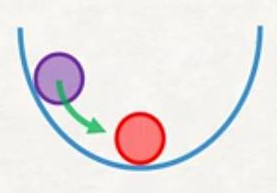
\includegraphics[width=10em]{phy_020_strs_04_01.jpg}

Yani top ilk denge konumuna dönecektir, ve o durumda potansiyel enerjisi minimum
olmuştur deriz ve bu denge stabil bir dengedir.


\includegraphics[width=10em]{phy_020_strs_04_02.jpg}

İkinci durumda topu orta noktada sola taşırız, top orada kalır, bu yeni
bir denge noktasıdır, $\Pi$ değişmemiştir, burada nötr bir denge vardır.

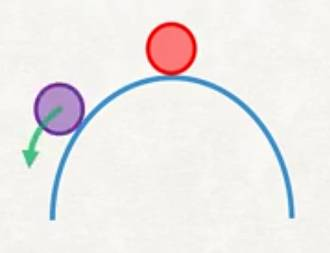
\includegraphics[width=10em]{phy_020_strs_04_03.jpg}

Üçüncü durumda ters kavisli bir yüzey var, top üst orta noktadan başlıyor
diyelim (orada durması zor olsa da), topu yine alıp sola taşıyorum, top aşağı
düşecektir. Üstteki durum potansiyel enerjisinin maksimum olduğu bir durumdur,
sistem stabil değildir. Rayleigh-Ritz yönteminin amacı (potansiyel enerjinin
minimum olduğu) stabil denge durumunu hedefleyerek bir yaklaşık çözüme
ulaşmaktır.

Bunu nasıl yaparız? Daha önce belirttiğimiz potansiyel enerjinin iki bileşeni
var, ilki sistemin toplam iç gerilim (deformasyon) enerjisi. Gerilim enerji
{\em yoğunluğu} $\overline{U}$ genel olarak bir materyelin stres-gerilim eğrisinin
altındaki alan olarak hesaplanabilir.

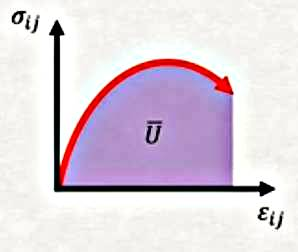
\includegraphics[width=10em]{phy_020_strs_04_04.jpg}

Mesela üstteki gibi stres $\sigma_{ij}$ ve gerilim $\epsilon_{ij}$ arasındaki
bir eğriyi düşünelim, bu eğrinin altında kalan alan, yani entegral hesabı 
gerilim enerji yoğunluğunu verir.

$$
\overline{U} = \int_{0}^{\epsilon_{ij}} \sigma_{ij} \ud \epsilon_{ij}
$$













[devam edecek]

Kaynaklar

[1] Petitt, {\em Intro to the Finite Element Method}, University of Alberta,
    \url{https://www.youtube.com/watch?v=2iUnfPRk6Ro&list=PLLSzlda_AXa3yQEJAb5JcmsVDy9i9K_fi}

\end{document}
